% =====================================================================
%  PETase-ML — Two-stage, leakage-audited protein-stability framework
%  SPRINGER NATURE (Scientific Reports) — sn-jnl template.
%
%  HOW TO USE ON OVERLEAF
%   1. On Overleaf choose:  New Project -> Templates ->
%      "Springer Nature LaTeX Template" (this provides sn-jnl.cls and the
%      Nature bibliography style). Open its example project.
%   2. Replace the template's main .tex with THIS file.
%   3. Add the file  sn-bibliography.bib  (provided) to the project.
%   4. Upload the figure  precision_vs_threshold.pdf  to the project root.
%   5. Compile with pdfLaTeX (Overleaf runs BibTeX automatically).
%
%  YELLOW  [TO ADD: ...]  markers are genuine gaps to fill/confirm before
%  submission. NOTE: Springer Nature does not render coloured text in the
%  final typeset XML, so REMOVE every yellow marker before final submission.
%
%  SCOPE (editorial, not printed): temperature-focused study; pH analysis and
%  EpHod excluded (future work only); general protein-stability framework
%  evaluated for potential PET-degrading-enzyme application (not PETase-specific
%  training data); no wet-lab/industrial/environmental claims; the older
%  19,071-mutation results are superseded and must not appear.
% =====================================================================
\documentclass[sn-nature]{sn-jnl}% Nature Portfolio reference style
% Alternatives if your journal differs: [sn-basic], [sn-mathphys-num], [sn-vancouver].

\usepackage{xcolor}
\usepackage{graphicx}
\usepackage{booktabs}

% ---- highlighted "to add" markers (remove before final submission) --
\newcommand{\todo}[1]{\colorbox{yellow}{\textbf{[TO ADD: #1]}}}
\newcommand{\todoblock}[1]{%
  \par\smallskip\noindent
  \colorbox{yellow}{\parbox{\dimexpr\linewidth-2\fboxsep\relax}{%
    \small\textbf{[TO ADD]}\ #1}}\par\smallskip}

% ---- shorthand ------------------------------------------------------
\newcommand{\ddg}{\ensuremath{\Delta\Delta G}}
\newcommand{\Tm}{\ensuremath{T_\mathrm{m}}}
\newcommand{\dtm}{\ensuremath{\Delta T_\mathrm{m}}}

\raggedbottom

\begin{document}

\title[Two-stage leakage-audited screening of PET-degrading enzymes]{A Two-Stage,
Leakage-Audited Machine-Learning Framework for Temperature- and Stability-Aware
Screening of PET-Degrading Enzymes}

% NOTE: confirm whether UC Santa Cruz is Ayush Iyer's institutional affiliation
% or a compute-resource acknowledgement only. Add James Ponzio's email if desired.
\author*[1]{\fnm{Ayush} \sur{Iyer}}\email{iyer.ayush31@gmail.com}
\author[2]{\fnm{James} \sur{Ponzio}}
\author[3]{\fnm{Abhinav} \sur{Iyer}}\email{abhinaviyer555@gmail.com}

\affil*[1]{\orgname{University of California, Santa Cruz}, \orgaddress{%
  \city{Santa Cruz}, \state{California}, \country{USA}}}
\affil[2]{\orgname{[TO ADD: James Ponzio -- department, organization, city, state, country]}}
\affil[3]{\orgname{[TO ADD: Abhinav Iyer -- department, organization, city, state, country]}}

% =====================================================================
\abstract{Plastic pollution is a defining environmental challenge, and enzymatic
depolymerization of polyethylene terephthalate (PET) offers a biological route to
recycling; however, candidate enzymes must remain stable under demanding conditions, and
computational screening is frequently inflated by data leakage. We built a general
protein-stability framework and evaluated it for potential application to PET-degrading
enzyme engineering. We assembled 1{,}001{,}888 mutation and stability records from seven
public sources and routed them by measurement type into a two-stage design: Stage~1
screens whole-protein thermostability (melting temperature, \Tm) and Stage~2 optimizes
mutation-level folding stability (\ddg). Training records were audited for exact and
sequence-homology leakage against the independent benchmarks. On the independent BRENDA
benchmark, Stage~1 reached a receiver-operating-characteristic (ROC) AUC of 0.732 (95\%
CI 0.708--0.755). On the independent S669 benchmark, Stage~2 reached a ROC AUC of 0.669
(95\% CI 0.62--0.72) and an ensemble Pearson correlation of 0.390 (95\% CI 0.32--0.46).
Both stages showed a precision--recall trade-off in which precision rose and recall fell
under stricter thresholds. These results describe a moderate, leakage-controlled
screen-then-optimize framework suited to prioritizing candidates for experimental
testing, not a validated industrial solution.}

\keywords{protein stability, machine learning, enzyme engineering, thermostability,
mutation-effect prediction, PET-degrading enzymes}

\maketitle

% =====================================================================
\section{Introduction}\label{sec:intro}
Polyethylene terephthalate (PET) is among the most heavily produced synthetic polymers,
and its accumulation as waste is a major contributor to global plastic pollution: global
plastics production reached roughly 460 million tonnes in 2019 and continues to rise, while
only a small fraction is recycled \cite{oecd2022plastics}.
% CONFIRM: verify the exact OECD figure/year and add any PET-specific value.
Biological recycling, in which
enzymes depolymerize PET into recoverable monomers, is an attractive complement to
mechanical and chemical recycling \cite{yoshida2016}.

Enzymatic PET degradation has advanced through the discovery and engineering of PET
hydrolases such as PETase and related cutinases \cite{yoshida2016,tournier2020,lu2022}.
Thermostability matters because reactions run faster near PET's glass-transition
temperature, but it is not the sole determinant of catalytic performance: activity,
substrate binding, reaction conditions, polymer crystallinity, and pH also matter.

Computational stability prediction addresses two related but non-interchangeable
questions. Whole-protein screening asks whether a given enzyme is thermostable,
summarized by its melting temperature (\Tm). Mutation-level optimization asks how a
specific substitution changes folding stability, expressed as the change in unfolding
free energy (\ddg). Conflating the two leads to misleading claims about what a model can
do.

A recurring problem in this literature is data leakage. Exact-match leakage (identical
sequences or mutations shared between training and test) and, more subtly,
sequence-homology leakage (shared homologous background) can inflate benchmark
performance. We do not claim that all prior models contain leakage; rather, we control
for it explicitly and report the effect.

Because whole-protein selection and mutation-level optimization are usually treated
separately, this study evaluates a single, integrated two-stage screen-then-optimize
framework---a general protein-stability method assessed for potential application to
PET-degrading enzyme engineering---on leakage-audited, independent BRENDA (temperature)
and S669 (\ddg) benchmarks, and reports its performance without overstating readiness.

% =====================================================================
\section{Results}\label{sec:results}

\subsection{Dataset composition and leakage auditing}\label{sec:data}
After harmonization, the multi-source staging table comprised 1{,}001{,}888 mutation and
stability records drawn from seven public sources (Table~\ref{tab:data}, Panel~A). Because
the framework treats temperature stability and folding stability as distinct problems,
records were routed by measurement type (Table~\ref{tab:data}, Panel~B): 29{,}654
melting-temperature (\Tm) records were assigned to Stage~1 and 508{,}693 folding
free-energy change (\ddg) records to Stage~2. Abundance-proxy (457{,}943) and \dtm{}
(5{,}598) records were retained in the table but were not used for model training.

To prevent optimistic bias, every candidate training record was audited against the
independent test proteins at two levels: exact-match (identical sequence and mutation)
and sequence-homology (shared homologous background). Auditing removed approximately
132{,}000 records, of which 131{,}479 were flagged by homology alone and would have been
invisible to exact-match filtering. This indicates that homology-level leakage, rather
than duplicate records, is the dominant contamination risk in this setting.

\subsection{Stage 1: temperature-stability performance on BRENDA}\label{sec:stage1}
\emph{Internal validation (development only).} During development, the Stage~1 temperature
model achieved an internal held-out root-mean-square error (RMSE) of approximately
6.5\,$^{\circ}$C and a validation Pearson correlation of approximately 0.80. These figures
describe performance on data drawn from the training distribution and characterize model
fitting only; they are not evidence of generalization and are reported separately from the
independent results below.

\emph{Independent testing (BRENDA benchmark).} Independent evaluation used a curated BRENDA
whole-protein temperature-stability benchmark \cite{chang2021brenda}. During curation, 412
records were removed to yield 2{,}034 proteins; a further 471 ambiguous cases were
excluded, leaving 1{,}563 proteins (979 positive, 584 negative). On this independent set
the classifier reached a ROC AUC of 0.732 (95\% CI 0.708--0.755). Evaluated as a regressor
against measured \Tm, it obtained a Pearson correlation of 0.54 (95\% CI 0.50--0.57),
rising to 0.60 on the subset with directly measured true-\Tm{} values
(Table~\ref{tab:stage1}).

\emph{Threshold behaviour.} Classification performance depended strongly on the decision
threshold (Fig.~\ref{fig:precision}a). As the temperature cutoff was made more stringent,
precision increased while recall fell---from 0.65 (recall 0.98) at the most permissive
cutoff to 0.93 (recall 0.39) and 0.98 (recall 0.32) at the strictest cutoffs
(Table~\ref{tab:stage1}, Panel~A). We emphasize that precision at a strict threshold is not
an experimental success rate: the 0.93 precision corresponds to only 39\% recall, so the
strict-threshold regime identifies a small, high-confidence set of stabilizing candidates
while missing most true positives.

\subsection{Stage 2: mutation-level \texorpdfstring{\ddg}{ddG} performance on S669}\label{sec:stage2}
Independent folding-stability performance was assessed on the S669 benchmark of 669 single
mutations (168 stabilizing, 501 non-stabilizing reference cases) \cite{pancotti2022s669}.
Across 2{,}000 bootstrap resamples, the gradient-boosted ensemble achieved an ensemble
Pearson correlation of 0.390 (95\% CI 0.32--0.46), RMSE 1.509\,kcal\,mol$^{-1}$, and a ROC
AUC of 0.669 (95\% CI 0.62--0.72) for stabilizing/non-stabilizing classification
(Table~\ref{tab:stage2}, Panels~A--B). Among individual models, Extra Trees---not the
ensemble---produced the strongest single-model regression metrics (Pearson 0.436;
Table~\ref{tab:stage2}, Panel~A).

As in Stage~1, precision and recall traded off with threshold stringency
(Fig.~\ref{fig:precision}b; Table~\ref{tab:stage2}, Panels~B--C). At the strict threshold
the ensemble reached precision 0.81 at only 10\% recall. The model therefore operates as a
high-precision, low-recall filter at strict cutoffs: the top-ranked candidates are enriched
for true stabilizers, but the majority of stabilizing mutations are not recovered. We
report this low recall explicitly rather than obscuring it, because it defines the model's
intended use as a candidate-prioritization filter.

\subsection{Cross-stage comparison}\label{sec:compare}
Stage~1 achieved a higher independent ROC AUC (0.732) than Stage~2 (0.669; Fig.~\ref{fig:roc}). However, the
two stages were trained and evaluated on different datasets, prediction targets
(temperature stability vs.\ folding \ddg), class labels, and sample sizes (1{,}563 vs.\ 669
records). The comparison is therefore descriptive only: it is not a controlled
head-to-head evaluation, and no statistical significance test was performed between the two
stages.
Positive (thermostable) proteins were defined as those with a derived stable-temperature
ceiling $\geq 60\,^{\circ}$C and negative proteins as those $\leq 45\,^{\circ}$C; proteins in
the intervening 45--60\,$^{\circ}$C band were treated as ambiguous and excluded (471
proteins), leaving 1{,}563 (979 positive, 584 negative) from 2{,}034 curated proteins, which
were themselves drawn from a pre-curation labeled set of 2{,}446. The $r=0.60$ regression
correlation was computed on the 325 curated proteins whose reported value is a directly
measured melting temperature (as opposed to a stability ceiling inferred from inactivation or
qualitative stability evidence). For \ddg, negative values denote stabilization; a variant is
predicted stabilizing when its predicted \ddg{} falls below the decision threshold, and
thresholds were swept from $-1.5$ to $+1.0$\,kcal\,mol$^{-1}$ to characterize the
precision--recall trade-off rather than to select an operating point on the benchmark.
% CONFIRM: the 325-subset matches the regression evaluation set, and thresholds were fixed before evaluation.

% =====================================================================
\section{Discussion}\label{sec:discussion}
The two-stage framework provides a moderate, leakage-controlled route from whole-protein
screening to mutation-level optimization. Stage~1's independent ROC AUC of 0.732 indicates
useful but imperfect discrimination of thermostable proteins, and its precision--recall
trade-off means the operating point should be chosen to match the intended use (broad
recall for discovery vs.\ high precision for shortlisting).

Stage~2's independent performance (Pearson 0.390; RMSE 1.509\,kcal\,mol$^{-1}$; ROC AUC
0.669) is best described as moderate, with pronounced high-precision/low-recall behaviour
at strict \ddg{} thresholds. This makes the model a candidate-prioritization filter rather
than a comprehensive predictor of every stabilizing mutation.

The central methodological contribution is explicit leakage auditing. Removing
approximately 132{,}000 records---the great majority (131{,}479) detectable only through
sequence homology---shows that homology-level contamination, not duplicate records, is the
dominant risk to honest benchmarking in this setting. A residual homology risk remains and
is acknowledged rather than dismissed.

Comparisons with prior \Tm{} or \ddg{} predictors are only meaningful when the benchmark,
sign convention, data split, and metric are matched; on S669, a broad set of stability
predictors has been benchmarked under matched conditions \cite{pancotti2022s669}. We therefore
restrict quantitative
comparison to genuinely comparable settings and avoid implying superiority across
incomparable evaluations.

We further caution that benchmark precision may not transfer unchanged to PET-degrading
enzymes, which are under-represented in these general stability sets. In particular, a
benchmark precision value such as 0.93 should not be equated with a 93\% experimental
success rate; it is measured at a chosen threshold on curated data, not in the laboratory.

Limitations include the moderate correlation on S669, the low recall at high-precision
operating points, the sequence-based (rather than structure-based) scope, residual
homology risk, and the fact that both benchmarks are general stability sets rather than
PET-hydrolase-specific assays. Future work should include PET-enzyme-specific evaluation,
incorporation of a pH-optimum analysis once a confirmed training run is available, and,
ultimately, experimental validation before any deployment claim.

% =====================================================================
\section{Methods}\label{sec:methods}

\subsection{Study design}
The framework comprises two stages that use different prediction targets and different data
subsets: Stage~1 (whole-protein \Tm) and Stage~2 (mutation-level \ddg). The full
1{,}001{,}888-record table did not train both models; records were routed by measurement
type (Table~\ref{tab:data}, Panel~B).

\subsection{Source datasets}
Records were drawn from seven public sources spanning both measurement types
(Table~\ref{tab:data}, Panel~A): the Human Domainome abundance dataset
\cite{beltran2025domainome}; the Tsuboyama et al.\ mega-scale folding-stability dataset and
its double-mutant subset \cite{tsuboyama2023}; the Meltome Atlas \cite{jarzab2020meltome};
ThermoMutDB \cite{xavier2021thermomutdb}; FireProtDB \cite{stourac2021fireprotdb}; and the
S2648 stability dataset \cite{dehouck2009s2648}. Independent evaluation used the BRENDA
enzyme benchmark \cite{chang2021brenda} for Stage~1 and the S669 benchmark
\cite{pancotti2022s669} for Stage~2; protein sequences were resolved through UniProt. The
Tsuboyama and Domainome data were obtained from their Zenodo deposits (records 7992926 and
13629491, respectively), and the BRENDA temperature-stability labels were parsed from the
BRENDA 2026.1 release. Per-source row counts and measurement-type allocation are given in
Table~\ref{tab:data}. The source datasets were downloaded and assembled between April and June
2026, and each was used under its respective public license (BRENDA under CC~BY~4.0); the
primary publication and repository or accession for each source are cited above and listed in
Table~\ref{tab:data}.
% CONFIRM: the exact license of each source, and the ProDDG/S2648 provenance (S2648 = Dehouck et al.).

\subsection{Harmonization and sequence resolution}
Records were harmonized to a common schema, typed by measurement, de-duplicated, and mapped
to canonical UniProt sequences retrieved through the UniProt REST API
(\texttt{rest.uniprot.org}) in June 2026 (training-set sequences on 18~June~2026 and BRENDA
benchmark sequences on 22~June~2026).
% CONFIRM: access dates (from fetch-output file timestamps); add canonical vs. isoform handling, failed-mapping count, and dedup policy.

\subsection{Leakage auditing}
Every candidate training record was audited against the independent benchmark proteins using
(i) an exact-key and mutation-level overlap check and (ii) a sequence-homology search with
MMseqs2 \cite{steinegger2017mmseqs2}. Searches were run with \texttt{mmseqs easy-search} at
maximum sensitivity ($-s\ 7.5$, $-e\ 1000$, \texttt{-{}-max-seqs 500}), and a training record
was flagged as leakage when it matched a benchmark protein at $\geq$30\% sequence identity
over $\geq$50\% query coverage (applied bidirectionally). From 1{,}135{,}644 stability-relevant
candidate records, the audit removed 2{,}627 exact duplicate measurements and 132{,}205 records
that matched the S669 test set; of the test-set matches, 131{,}536 were flagged by sequence
homology and the remainder by exact keys (300 by UniProt-plus-mutation, 232 by wild-type
sequence hash, 70 by PDB-plus-chain-plus-mutation, and 67 by PDB-plus-mutation), with 131{,}479
of the homology matches invisible to every exact key. This left 1{,}001{,}888 training-eligible
records.

\subsection{Features}
Proteins and mutations were represented using ESM-2 protein-language-model embeddings
\cite{lin2023esm2}. Per-residue representations were taken from the final layer of
\texttt{esm2\_t30\_150M\_UR50D} (640 dimensions) and mean-pooled over the sequence. For the
Stage~1 whole-protein model the feature vector was the mean-pooled embedding together with
the log sequence length; for the Stage~2 mutation model the features combined the wild-type
and mutant mean-pooled embeddings and their difference
($[\mathbf{e}_{wt},\ \mathbf{e}_{mut},\ \mathbf{e}_{mut}-\mathbf{e}_{wt}]$) with an ESM-2
log-likelihood-ratio score for the substitution. These embedding features were reduced by
principal component analysis to 256 dimensions before the boosting models.
% CONFIRM: final feature set and PCA dimensionality (GPU job runs build_features.py --pca 256); embedding model esm2_t30_150M_UR50D (some earlier scripts use esm2_t12_35M); do not carry features from the 19,071-mutation model.

\subsection{Models and ensemble}
Each stage used an ensemble that averaged the predictions of its base models, all with a
fixed random seed of 42. Stage~1 (\Tm) combined Extra Trees and Random Forest (400 trees,
maximum depth 25), XGBoost \cite{chen2016xgboost} (600 rounds, depth 6, learning rate 0.03),
LightGBM \cite{ke2017lightgbm} (800 rounds, learning rate 0.03), and CatBoost
\cite{prokhorenkova2018catboost} (800 iterations, depth 8, learning rate 0.03). Stage~2 (\ddg)
combined Random Forest and Extra Trees (300 trees, maximum depth 25), a multilayer perceptron
(up to 100 iterations), XGBoost (600 rounds, depth 9, learning rate 0.02, subsample 0.8,
histogram tree construction on GPU), LightGBM, and CatBoost (GPU training). Random Forest,
Extra Trees, and the multilayer perceptron were implemented in scikit-learn
\cite{pedregosa2011sklearn}. The ensemble prediction was the unweighted mean of the
base-model outputs.

\subsection{Evaluation}
Models were trained on a protein-grouped training/validation split (grouped so that no
protein spanned both partitions; seed 42) and evaluated on the held-out, leakage-audited
BRENDA and S669 benchmarks. Classification was summarized by ROC AUC, precision, recall, F1,
and accuracy across decision thresholds; regression by Pearson and Spearman correlation and
RMSE. Confidence intervals were estimated by bootstrapping the test items with replacement
(2{,}000 resamples; percentile 95\% CI; seed 0), reusing the saved per-item predictions
without retraining. Software: Python 3.10 with PyTorch 2.1.0 (CUDA 12.1), fair-esm 2.0.0,
scikit-learn 1.7.2, XGBoost 3.2.0, LightGBM 4.7.0, CatBoost 1.2.10, NumPy 1.26, and pandas
2.3.3. GPU components were trained on the National Research Platform (Nautilus) Kubernetes
cluster using the \texttt{pytorch/pytorch:2.1.0-cuda12.1-cudnn8-runtime} container
(\texttt{large-gpu} partition); sequence-homology auditing used MMseqs2 release~18-8cc5c.
% CONFIRM: these versions were reproduced from the training container (original run unpinned); confirm with a pinned re-run.

% =====================================================================
\backmatter

\bmhead{Supplementary information}
Not applicable; all display items are included in the main text.

\bmhead{Acknowledgements}
The authors thank the National Research Platform (Nautilus) for providing computational
resources. Nautilus is supported by the Pacific Research Platform (NSF award~1541349),
CHASE-CI (NSF award~1730158), and Towards a National Research Platform (NSF award~1826967),
with additional funding from the University of California Office of the President.
% CONFIRM: verify these NRP/NSF award numbers are current for your usage, and add any
% individual (non-author) acknowledgements with their consent.

\section*{Declarations}
\begin{itemize}
  \item \textbf{Funding.}\ No specific grant funding was received for this work; computational
        resources were provided by the National Research Platform (Nautilus).
        % CONFIRM funding status with all authors (change if a grant supported the work).
  \item \textbf{Competing interests.}\ The authors declare no competing interests.
        % CONFIRM with all authors before submission.
  \item \textbf{Ethics approval and consent to participate.}\ Not applicable (computational study using public data).
  \item \textbf{Consent for publication.}\ Not applicable.
  \item \textbf{Data availability.}\ The processed training table, leakage-audited benchmark
        datasets, saved predictions, split identifiers, leakage-audit outputs, and trained
        model artifacts generated in this study are available through Zenodo
        (\url{https://doi.org/10.5281/zenodo.21257369}); source datasets are cited above.
        % ACTION before submission: make the Zenodo record open (or provide reviewer access)
        % and apply a data license such as CC BY 4.0 instead of the current GPL-3.0; confirm
        % the deposit contains all listed artifacts with a README/data dictionary.
  \item \textbf{Materials availability.}\ Not applicable.
  \item \textbf{Large-language-model use.}\ A large language model (Anthropic Claude) was used
        to assist with drafting, formatting, and reference preparation; all content was
        reviewed and verified by the authors, who take full responsibility for it.
        % CONFIRM wording against the journal's current LLM-use policy.
  \item \textbf{Code availability.}\ Source code for data assembly, leakage auditing, model
        training, evaluation, threshold analysis, bootstrap confidence-interval estimation,
        and figure generation is available at \url{https://github.com/AyushIyer31/PET-Lab}
        and archived on Zenodo at \url{https://doi.org/10.5281/zenodo.21519961} (release
        v1.0.0).
        % CONFIRM the archived commit (497c4f5) is the exact code that produced the results,
        % and that a README, license, environment file, seeds, and reproduction commands exist.
  \item \textbf{Author contributions.}\ (Provisional --- authors to confirm.) A.I.\ contributed
        to conceptualization, software, data curation, formal analysis, investigation,
        methodology, visualization, and writing of the original draft. J.P.\ contributed to
        conceptualization, supervision, validation, and writing (review and editing). Ab.I.\
        contributed to investigation, writing of the original draft, and writing (review and
        editing). All authors reviewed and approved the final manuscript.
        % CONFIRM/ADJUST the CRediT roles above and the author order before submission.
\end{itemize}

% =====================================================================
% ============================ DISPLAY ITEMS ==========================
% =====================================================================

\begin{table}[htbp]
\caption{Composition of the assembled dataset and allocation by measurement type. Exact
record counts; both panels sum to 1{,}001{,}888.}\label{tab:data}
\centering
\small
\begin{tabular}{@{}lr@{}}
\toprule
\multicolumn{2}{@{}l}{\textit{Panel A --- Rows by source dataset}}\\
\midrule
Source dataset & Rows\\
\midrule
Domainome (aPCA abundance)              & 457{,}943\\
Tsuboyama et al.\ 2023 (mega-scale)     & 357{,}155\\
Tsuboyama et al.\ 2023 (double mutants) & 138{,}275\\
Meltome Atlas                           & 27{,}884\\
ThermoMutDB                             & 11{,}520\\
FireProtDB                              & 6{,}549\\
ProDDG/S2648                            & 2{,}562\\
\midrule
Total                                   & 1{,}001{,}888\\
\botrule
\end{tabular}

\vspace{6pt}
\begin{tabular}{@{}lrl@{}}
\toprule
\multicolumn{3}{@{}l}{\textit{Panel B --- Rows by measurement type and model allocation}}\\
\midrule
Measurement type & Rows & Used to train\\
\midrule
\ddg{} (mutation)     & 508{,}693 & Stage 2\\
Abundance (proxy)     & 457{,}943 & Not used in this study\\
\Tm{} (whole protein) & 29{,}654  & Stage 1\\
\dtm{}                & 5{,}598   & Not used in this study\\
\midrule
Total                 & 1{,}001{,}888 & ---\\
\botrule
\end{tabular}
\end{table}

\begin{table}[htbp]
\caption{Stage 1 melting-temperature model: classification on the independent BRENDA
benchmark (1{,}563 enzymes; 979 positive, 584 negative). Positive class $=$ thermostable.
ROC AUC $=0.732$ (95\% CI 0.708--0.755). Precision is reported with recall, F1, and accuracy
so that it is not read as overall reliability.}\label{tab:stage1}
\centering
\small
\begin{tabular}{@{}lcccc@{}}
\toprule
\multicolumn{5}{@{}l}{\textit{Panel A --- Decision-threshold analysis}}\\
\midrule
Threshold & Precision & Recall & F1 & Accuracy\\
\midrule
46\,$^{\circ}$C & 0.65 & 0.98 & 0.78 & 0.66\\
50\,$^{\circ}$C & 0.71 & 0.77 & 0.74 & 0.66\\
52\,$^{\circ}$C & 0.77 & 0.63 & 0.69 & 0.65\\
60\,$^{\circ}$C & 0.93 & 0.39 & 0.55 & 0.60\\
66\,$^{\circ}$C & 0.98 & 0.32 & 0.49 & 0.58\\
\botrule
\end{tabular}

\vspace{6pt}
\begin{tabular}{@{}lccc@{}}
\toprule
\multicolumn{4}{@{}l}{\textit{Panel B --- Per-model performance at the 60\,$^{\circ}$C threshold}}\\
\midrule
Model & Precision & Recall & F1\\
\midrule
Extra Trees   & 0.963 & 0.369 & 0.533\\
Random Forest & 0.948 & 0.355 & 0.517\\
LightGBM      & 0.933 & 0.395 & 0.555\\
CatBoost      & 0.927 & 0.400 & 0.559\\
XGBoost       & 0.917 & 0.394 & 0.551\\
Ensemble      & 0.945 & 0.388 & 0.550\\
\botrule
\end{tabular}
\end{table}

\begin{table}[htbp]
\caption{Stage 2 mutation-level \ddg{} model: regression and classification on the
independent S669 benchmark (669 mutations; 168 stabilizing, 501 non-stabilizing reference
cases). Ensemble ROC AUC $=0.669$ (95\% CI 0.62--0.72); ensemble regression Pearson $=0.390$
(95\% CI 0.32--0.46); 2{,}000 bootstrap resamples.}\label{tab:stage2}
\centering
\small
\begin{tabular}{@{}lccc@{}}
\toprule
\multicolumn{4}{@{}l}{\textit{Panel A --- Regression (predicted vs.\ experimental \ddg)}}\\
\midrule
Model & Pearson & Spearman & RMSE (kcal\,mol$^{-1}$)\\
\midrule
Extra Trees           & 0.436 & 0.461 & 1.481\\
XGBoost               & 0.382 & 0.413 & 1.514\\
Random Forest         & 0.369 & 0.396 & 1.523\\
LightGBM              & 0.330 & 0.364 & 1.549\\
CatBoost              & 0.324 & 0.362 & 1.557\\
Multilayer perceptron & 0.298 & 0.338 & 1.612\\
Ensemble              & 0.390 & 0.414 & 1.509\\
\botrule
\end{tabular}

\vspace{6pt}
\begin{tabular}{@{}lcccc@{}}
\toprule
\multicolumn{5}{@{}l}{\textit{Panel B --- Ensemble classification across decision thresholds}}\\
\midrule
Threshold & Precision & Recall & F1 & Accuracy\\
\midrule
0.00\,kcal\,mol$^{-1}$   & 0.81 & 0.10 & 0.18 & 0.77\\
$+$0.25\,kcal\,mol$^{-1}$ & 0.51 & 0.26 & 0.35 & 0.75\\
$+$0.50\,kcal\,mol$^{-1}$ & 0.38 & 0.46 & 0.42 & 0.67\\
$+$1.00\,kcal\,mol$^{-1}$ & 0.31 & 0.80 & 0.45 & 0.51\\
\botrule
\end{tabular}

\vspace{6pt}
\begin{tabular}{@{}lcc@{}}
\toprule
\multicolumn{3}{@{}l}{\textit{Panel C --- Per-model performance at the strict (0.00\,kcal\,mol$^{-1}$) threshold}}\\
\midrule
Model & Precision & Recall\\
\midrule
Random Forest         & 0.900 & 0.107\\
Extra Trees           & 0.786 & 0.065\\
XGBoost               & 0.735 & 0.149\\
LightGBM              & 0.625 & 0.119\\
CatBoost              & 0.429 & 0.107\\
Multilayer perceptron & 0.415 & 0.202\\
Ensemble              & 0.810 & 0.101\\
\botrule
\end{tabular}
\end{table}

\begin{figure}[htbp]
\centering
\IfFileExists{precision_vs_threshold.pdf}{%
  
\includegraphics[width=\textwidth]{precision_vs_threshold.pdf}%
}{\IfFileExists{precision_vs_threshold.png}{%
  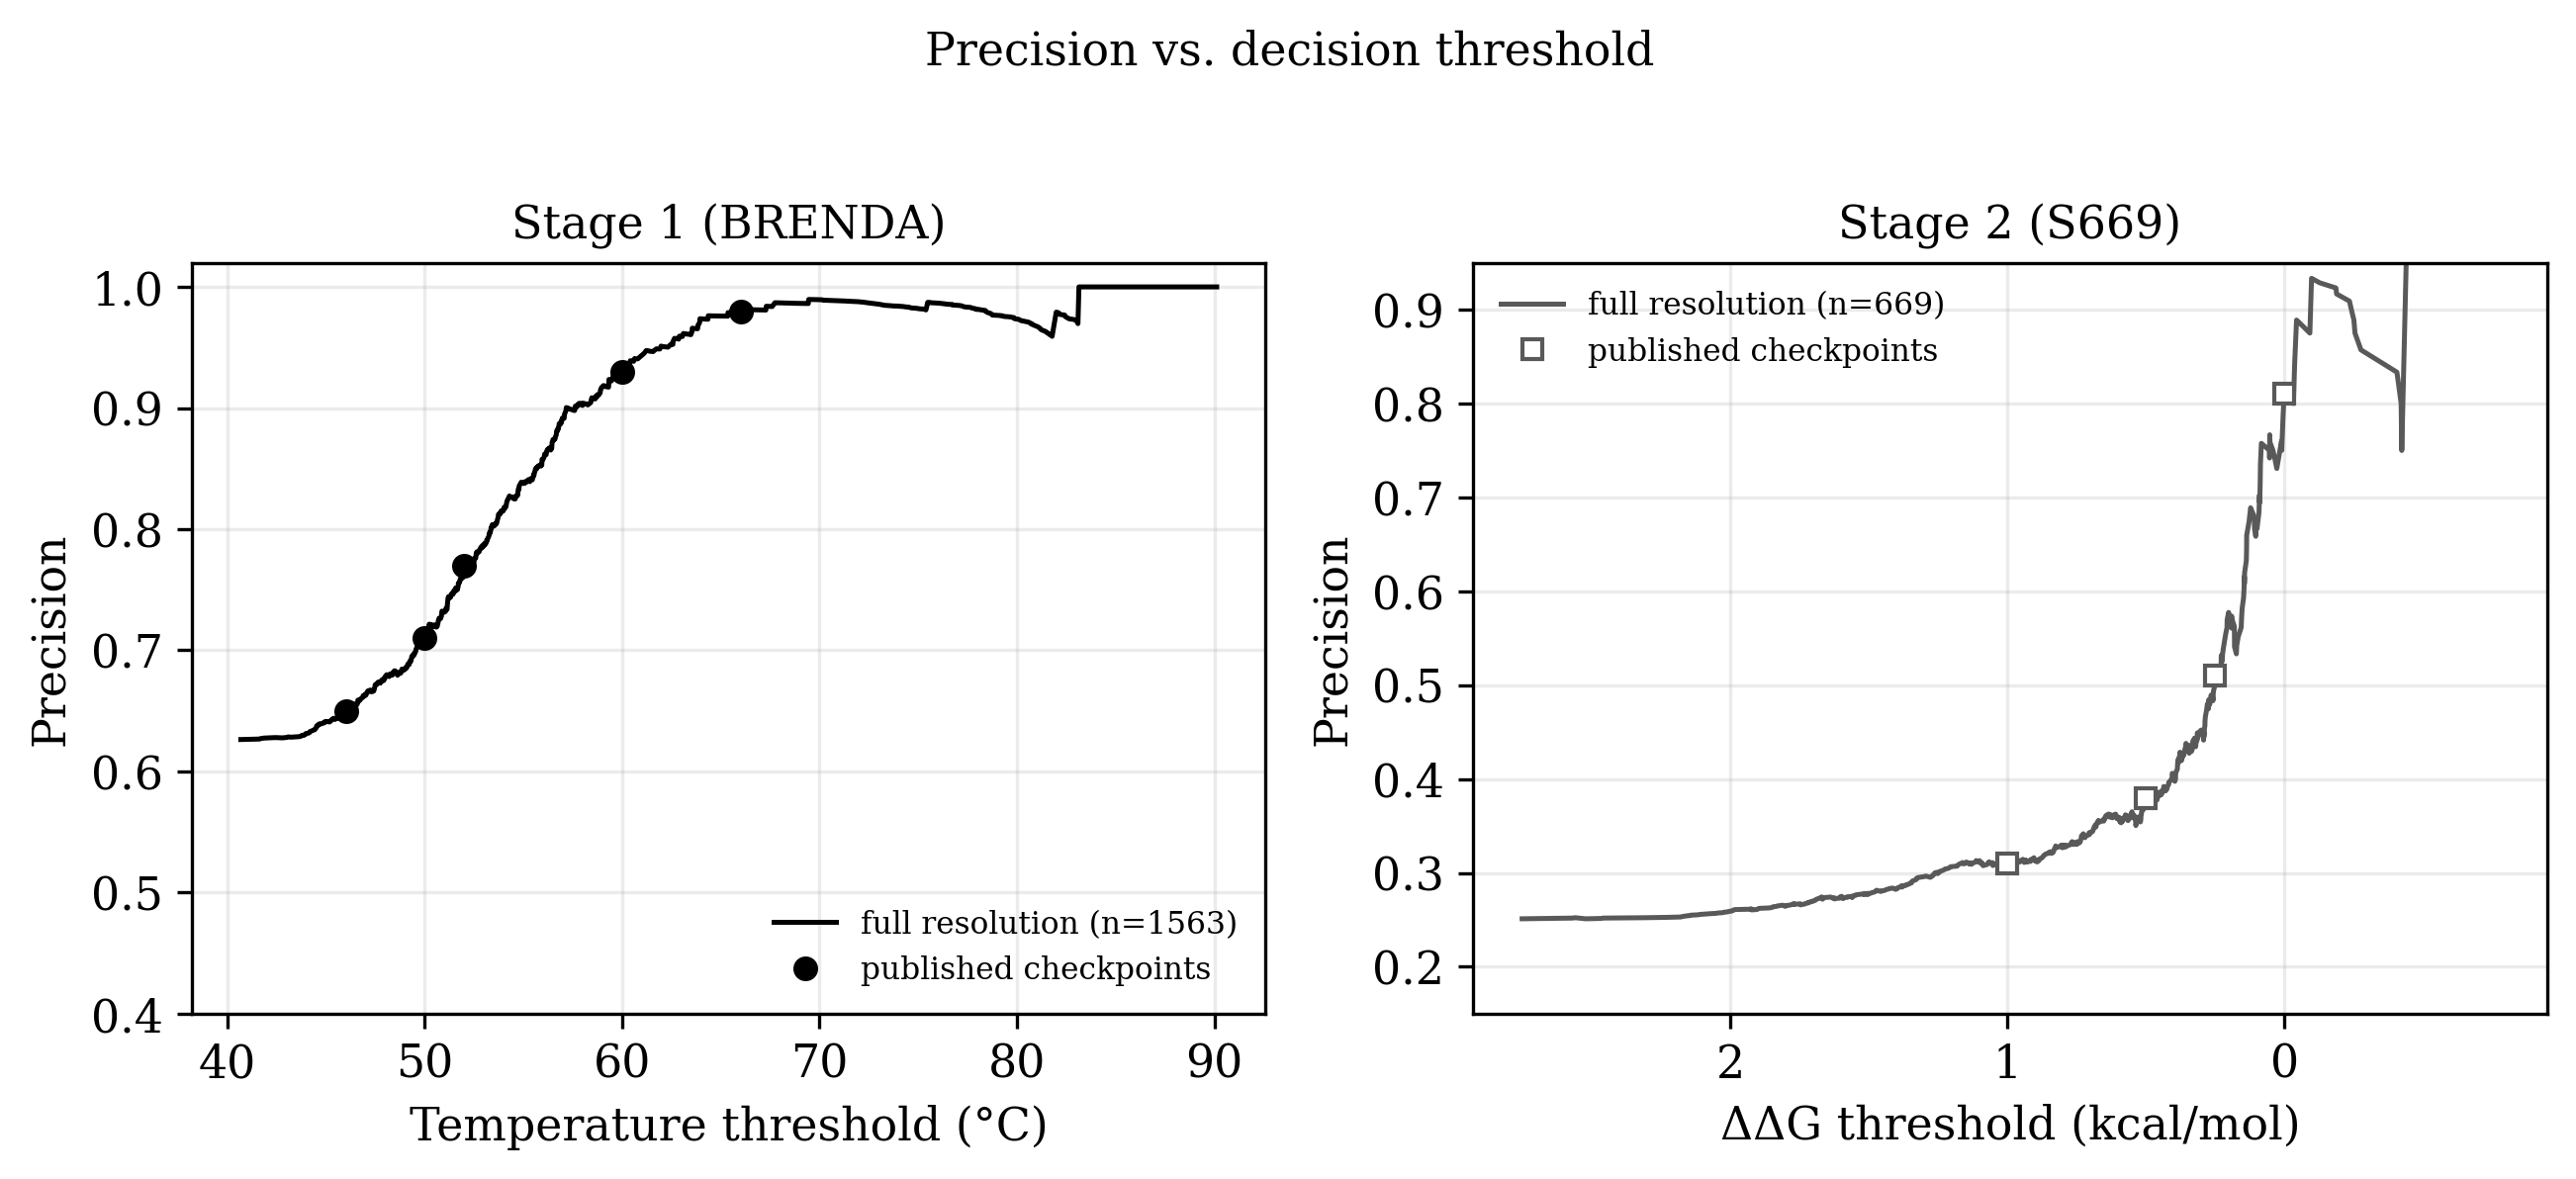
\includegraphics[width=\textwidth]{precision_vs_threshold.png}%
}{%
  \fbox{\parbox[c][0.32\textwidth][c]{0.95\textwidth}{\centering
    \todo{upload precision\_vs\_threshold.pdf (or .png) into the Overleaf project}}}%
}}
\caption{Precision as a function of the decision threshold for the two-stage framework on
independent benchmarks. Precision for the Stage~1 whole-protein melting-temperature model on
the leakage-audited BRENDA benchmark ($n=1{,}563$; 979 positive, 584 negative) across
melting-temperature thresholds (panel~a) and for the Stage~2 mutation-level \ddg{} model on
S669 ($n=669$; 168 stabilizing, 501 non-stabilizing reference cases) across \ddg{} thresholds
(panel~b). In both panels the horizontal axis is oriented so that precision increases with
more stringent thresholds. Recall, F1, accuracy, and ROC AUC for the same evaluations are
reported in Tables~\ref{tab:stage1}--\ref{tab:stage2}. Positive class: BRENDA $=$
thermostable; S669 $=$ stabilizing.}\label{fig:precision}
\end{figure}

\begin{figure}[htbp]
\centering
\IfFileExists{roc_curve.pdf}{%
  
\includegraphics[width=0.75\textwidth]{roc_curve.pdf}%
}{\IfFileExists{roc_curve.png}{%
  
\includegraphics[width=0.75\textwidth]{roc_curve.png}%
}{%
  \fbox{\parbox[c][0.32\textwidth][c]{0.95\textwidth}{\centering
    \todo{upload roc\_curve.pdf (or .png) into the Overleaf project}}}%
}}
\caption{Receiver-operating-characteristic (ROC) curves on the independent benchmarks:
Stage~1 (whole-protein \Tm) on BRENDA ($n=1{,}563$; ROC AUC 0.732) and Stage~2 (mutation-level
\ddg) on S669 ($n=669$; ROC AUC 0.669). Positive class: BRENDA $=$ thermostable; S669 $=$
stabilizing.}\label{fig:roc}
\end{figure}

% =====================================================================
% References embedded directly (no external .bib / BibTeX step needed).
% If you prefer BibTeX, delete this block and use \bibliography{sn-bibliography}.
\begin{thebibliography}{99}

\bibitem{oecd2022plastics}
OECD. \textit{Global Plastics Outlook: Economic Drivers, Environmental Impacts and Policy
Options} (OECD Publishing, Paris, 2022).

\bibitem{yoshida2016}
Yoshida, S. et al. A bacterium that degrades and assimilates poly(ethylene terephthalate).
\textit{Science} \textbf{351}, 1196--1199 (2016).

\bibitem{tournier2020}
Tournier, V. et al. An engineered PET depolymerase to break down and recycle plastic bottles.
\textit{Nature} \textbf{580}, 216--219 (2020).

\bibitem{lu2022}
Lu, H. et al. Machine learning-aided engineering of hydrolases for PET depolymerization.
\textit{Nature} \textbf{604}, 662--667 (2022).

\bibitem{chang2021brenda}
Chang, A. et al. BRENDA, the ELIXIR core data resource in 2021: new developments and updates.
\textit{Nucleic Acids Res.} \textbf{49}, D498--D508 (2021).

\bibitem{pancotti2022s669}
Pancotti, C. et al. Predicting protein stability changes upon single-point mutation: a thorough
comparison of the available tools on a new dataset. \textit{Brief. Bioinform.} \textbf{23},
bbab555 (2022).

\bibitem{beltran2025domainome}
Beltran, A., Jiang, X., Shen, Y. \& Lehner, B. Site-saturation mutagenesis of 500 human
protein domains. \textit{Nature} (2025). https://doi.org/10.1038/s41586-024-08370-4

\bibitem{tsuboyama2023}
Tsuboyama, K. et al. Mega-scale experimental analysis of protein folding stability in biology
and design. \textit{Nature} \textbf{620}, 434--444 (2023).

\bibitem{jarzab2020meltome}
Jarzab, A. et al. Meltome atlas---thermal proteome stability across the tree of life.
\textit{Nat. Methods} \textbf{17}, 495--503 (2020).

\bibitem{xavier2021thermomutdb}
Xavier, J. S. et al. ThermoMutDB: a thermodynamic database for missense mutations.
\textit{Nucleic Acids Res.} \textbf{49}, D475--D479 (2021).

\bibitem{stourac2021fireprotdb}
Stourac, J. et al. FireProtDB: database of manually curated protein stability data.
\textit{Nucleic Acids Res.} \textbf{49}, D319--D324 (2021).

\bibitem{dehouck2009s2648}
Dehouck, Y. et al. Fast and accurate predictions of protein stability changes upon mutations
using statistical potentials and neural networks: PoPMuSiC-2.0. \textit{Bioinformatics}
\textbf{25}, 2537--2543 (2009).

\bibitem{steinegger2017mmseqs2}
Steinegger, M. \& S\"oding, J. MMseqs2 enables sensitive protein sequence searching for the
analysis of massive data sets. \textit{Nat. Biotechnol.} \textbf{35}, 1026--1028 (2017).

\bibitem{lin2023esm2}
Lin, Z. et al. Evolutionary-scale prediction of atomic-level protein structure with a language
model. \textit{Science} \textbf{379}, 1123--1130 (2023).

\bibitem{chen2016xgboost}
Chen, T. \& Guestrin, C. XGBoost: a scalable tree boosting system. In \textit{Proc. 22nd ACM
SIGKDD Int. Conf. Knowledge Discovery and Data Mining}, 785--794 (2016).

\bibitem{ke2017lightgbm}
Ke, G. et al. LightGBM: a highly efficient gradient boosting decision tree. In \textit{Advances
in Neural Information Processing Systems} \textbf{30} (2017).

\bibitem{prokhorenkova2018catboost}
Prokhorenkova, L. et al. CatBoost: unbiased boosting with categorical features. In
\textit{Advances in Neural Information Processing Systems} \textbf{31} (2018).

\bibitem{pedregosa2011sklearn}
Pedregosa, F. et al. Scikit-learn: machine learning in Python. \textit{J. Mach. Learn. Res.}
\textbf{12}, 2825--2830 (2011).

\end{thebibliography}

\end{document}
